\documentclass[conference]{IEEEtran}

% ---------- Packages ----------
\usepackage{graphicx}
\usepackage{amsmath,amssymb}
\usepackage[hidelinks]{hyperref}
\usepackage{siunitx}
\usepackage{booktabs}
\usepackage[table]{xcolor}
\usepackage{tikz}
\usetikzlibrary{arrows.meta,positioning,shapes,fit}
\usepackage[section]{placeins} % 図のせり上がり防止(セクションごとにバリア)

% ---------- Title ----------
\title{AITL on Space: A Robust Three-Layer Architecture\\
with a Tri\,-NVM Hierarchy (SRAM / MRAM / FRAM)\\
for Long-Duration Spacecraft Autonomy}

\author{%
  \IEEEauthorblockN{Shinichi Samizo}
  \IEEEauthorblockA{Independent Semiconductor Researcher\\
  Former Engineer at Seiko Epson Corporation\\
  Email: \href{mailto:shin3t72@gmail.com}{shin3t72@gmail.com}\quad
  GitHub: \url{https://github.com/Samizo-AITL}}%
}

\begin{document}
\maketitle

% ---------- Abstract ----------
\begin{abstract}
We propose \emph{AITL on Space}, a three-layer control architecture (Robust Core, FSM Supervisor, AI Adaptor) implemented on a \SI{22}{nm} FDSOI SoC with a hardened \emph{Tri-NVM hierarchy} (SRAM / MRAM / FRAM). The system targets ultra-robust autonomy under radiation, thermal cycling, and long-term drift. This paper outlines the architecture, state-space model (8--20\,D), $H_\infty$ mixed-sensitivity design flow, and a verification pipeline from FPGA HIL to ASIC.
\end{abstract}
\FloatBarrier % ← ここより前に図が浮上しない

% ---------- 1. Introduction ----------
\section{Introduction}
Long-duration missions require high availability under TID/SEE and thermal cycles. Conventional PID\,+\,Flash architectures face reliability limits. We summarize related work and motivate AITL on Space.

% ---------- 2. System Architecture ----------
\section{System Architecture}
AITL comprises: (i) Robust Core ($H_\infty$/MPC/SMC), (ii) FSM Supervisor (Safe/Nominal/Recovery, FDI/FDII), and (iii) AI Adaptor for long-term re-identification. A \textbf{Tri-NVM hierarchy}---SRAM for execution, MRAM for logs/code (ECC\,+\,scrub, A/B slots), FRAM for safe boot---ensures persistence.

\begin{figure}[!t]
  \centering
  \resizebox{\columnwidth}{!}{%
    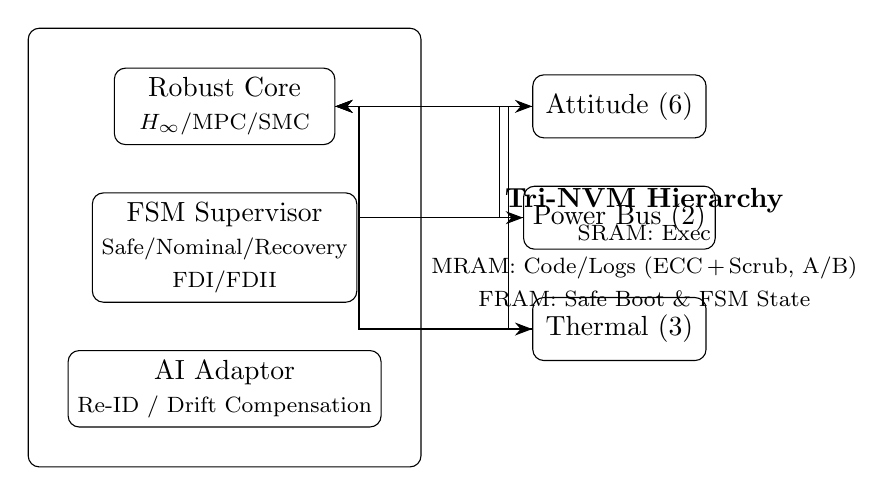
\begin{tikzpicture}[
      node distance=6mm and 10mm,
      box/.style={draw,rounded corners,minimum width=28mm,minimum height=8mm,align=center},
      mem/.style={draw,rounded corners,fill=gray!10,minimum width=22mm,minimum height=7mm,align=center},
      >={Stealth[length=2.2mm]}
    ]
      % Layers
      \node[box] (robust) {Robust Core\\ \footnotesize $H_\infty$/MPC/SMC};
      \node[box,below=of robust] (fsm) {FSM Supervisor\\ \footnotesize Safe/Nominal/Recovery\\ \footnotesize FDI/FDII};
      \node[box,below=of fsm] (ai) {AI Adaptor\\ \footnotesize Re-ID / Drift Compensation};

      % Memory block (Tri-NVM)
      \node[draw,rounded corners,fit={(robust) (fsm) (ai)},inner sep=5mm,label={[align=center]right:\textbf{Tri-NVM Hierarchy}\\
      \footnotesize SRAM: Exec\\
      \footnotesize MRAM: Code/Logs (ECC\,+\,Scrub, A/B)\\
      \footnotesize FRAM: Safe Boot \& FSM State}] (stack) {};

      % Plant blocks (attitude, power, thermal)
      \node[box,right=25mm of robust,minimum width=22mm] (att) {Attitude (6)};
      \node[box,below=of att,minimum width=22mm] (pwr) {Power Bus (2)};
      \node[box,below=of pwr,minimum width=22mm] (thm) {Thermal (3)};

      % Arrows to plant
      \draw[->] (robust.east) -- ++(3mm,0) |- (att.west);
      \draw[->] (robust.east) -- ++(3mm,0) |- (pwr.west);
      \draw[->] (robust.east) -- ++(3mm,0) |- (thm.west);

      % Feedback to robust
      \draw[->] (att.west) -- ++(-3mm,0) |- (robust.east);
      \draw[->] (pwr.west) -- ++(-3mm,0) |- (robust.east);
      \draw[->] (thm.west) -- ++(-3mm,0) |- (robust.east);
    \end{tikzpicture}
  }
  \caption{AITL on Space architecture with Robust Core, Supervisor FSM, AI Adaptor, and the Tri-NVM hierarchy.}
  \label{fig:arch_block}
\end{figure}

% ---------- 3. Mathematical Model ----------
\section{Mathematical Model}
We use an 11D PoC plant that couples attitude (6), power bus (2), and thermal nodes (3). The discrete-time model is
\begin{align}
x_{k+1} &= A x_k + B u_k + E w_k, \qquad
y_k = C x_k + D u_k + v_k .
\end{align}
Extensions scale to 20D with translational axes and bias states.

\begin{figure}[!t]
  \centering
  \resizebox{.9\columnwidth}{!}{%
    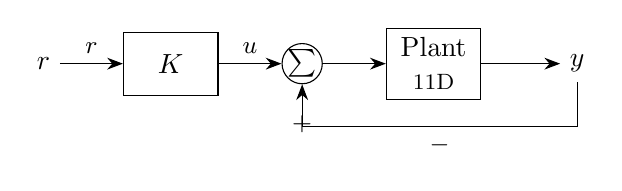
\begin{tikzpicture}[
      block/.style={draw,minimum width=12mm,minimum height=8mm,align=center},
      sum/.style={circle,draw,inner sep=0pt,minimum size=3.2mm},
      >={Stealth[length=2mm]}
    ]
      \node[block] (K) {$K$};
      \node[sum,right=8mm of K] (s) {$\sum$};
      \node[block,right=8mm of s] (P) {Plant\\ \footnotesize 11D};
      \node[right=10mm of P] (y) {$y$};

      \draw[->] (K) -- node[above]{\small $u$} (s);
      \draw[->] (s) -- (P) ;
      \draw[->] (P) -- (y);
      \draw[->] (y) |- ++(0,-8mm) -| node[pos=.25,below]{\small $-$} node[pos=.75,below]{\small $+$} (s);
      \node[left=8mm of K] (r) {$r$};
      \draw[->] (r) -- node[above]{\small $r$} (K);
    \end{tikzpicture}
  }
  \caption{Closed-loop schematic used for $H_\infty$ synthesis on the 11D plant.}
  \label{fig:state_space}
\end{figure}

% ---------- 4. H-infinity ----------
\section{$H_\infty$ Mixed-Sensitivity Design}
Weights $(W_1,W_2,W_3)$ shape sensitivity, effort, and complementary sensitivity. EduController exports JSON plant/weights; AITL-H synthesizes output-feedback $K$ and fixed-point realization.

% ---------- 5. Verification Pipeline ----------
\section{Verification Pipeline}
FPGA HIL injects SEU bursts and sensor outages; metrics include safe-mode time ($\leq \SI{1}{s}$), recovery rate ($\geq 99\%$), and ECC statistics. Physical design proceeds to 22FDX tape-out; SystemDK FEM closes thermal/packaging.

\begin{figure}[!t]
  \centering
  \resizebox{\columnwidth}{!}{%
    \begin{tikzpicture}[
      step/.style={draw,rounded corners,minimum width=23mm,minimum height=8mm,align=center},
      >={Stealth[length=2mm]}
    ]
      \node[step,fill=green!10] (json) {JSON\\Plant/Weights};
      \node[step,fill=green!10,below=6mm of json] (rtl) {RTL Synthesis};
      \node[step,fill=orange!10,below=6mm of rtl] (hil) {FPGA HIL};
      \node[step,fill=pink!10,below=6mm of hil] (asic) {22FDX ASIC};

      \node[step,fill=gray!15,right=28mm of hil,minimum width=35mm] (fem) {SystemDK FEM\\ \footnotesize Thermal / Radiation / Packaging};

      \draw[->] (json) -- (rtl);
      \draw[->] (rtl) -- (hil);
      \draw[->] (hil) -- (asic);
      \draw[->] (hil) -- (fem);
    \end{tikzpicture}
  }
  \caption{Verification pipeline from JSON design to RTL, FPGA HIL, and ASIC; SystemDK closes the loop with thermal and radiation scenarios.}
  \label{fig:pipeline}
\end{figure}

% ---------- 6. Conclusion ----------
\section{Conclusion}
AITL on Space offers a practical path to resilient autonomy for deep-space missions.

% ---------- References ----------
\bibliographystyle{ieeetr}
\begin{thebibliography}{9}
\bibitem{hinf} Doyle, G. \emph{et al.}, \emph{Feedback Control Theory}.
\bibitem{fds} Colinge, J.-P., \emph{Silicon-on-Insulator Technology}.
\end{thebibliography}

% ---------- Biography ----------
\section*{Author Biography}
\textbf{Shinichi Samizo} received the M.S. degree in Electrical and Electronic Engineering from Shinshu University, Japan. He worked at Seiko Epson Corporation as an engineer in semiconductor memory and mixed-signal device development, and contributed to inkjet MEMS actuators and PrecisionCore printhead technology. He is currently an independent semiconductor researcher focusing on process/device education, memory architecture, and AI system integration. Contact: \href{mailto:shin3t72@gmail.com}{shin3t72@gmail.com}.

\end{document}
